
%% bare_conf.tex
%% V1.4a
%% 2014/09/17
%% by Michael Shell
%% See:
%% http://www.michaelshell.org/
%% for current contact information.
%%
%% This is a skeleton file demonstrating the use of IEEEtran.cls
%% (requires IEEEtran.cls version 1.8a or later) with an IEEE
%% conference paper.
%%
%% Support sites:
%% http://www.michaelshell.org/tex/ieeetran/
%% http://www.ctan.org/tex-archive/macros/latex/contrib/IEEEtran/
%% and
%% http://www.ieee.org/

%%*************************************************************************
%% Legal Notice:
%% This code is offered as-is without any warranty either expressed or
%% implied; without even the implied warranty of MERCHANTABILITY or
%% FITNESS FOR A PARTICULAR PURPOSE! 
%% User assumes all risk.
%% In no event shall IEEE or any contributor to this code be liable for
%% any damages or losses, including, but not limited to, incidental,
%% consequential, or any other damages, resulting from the use or misuse
%% of any information contained here.
%%
%% All comments are the opinions of their respective authors and are not
%% necessarily endorsed by the IEEE.
%%
%% This work is distributed under the LaTeX Project Public License (LPPL)
%% ( http://www.latex-project.org/ ) version 1.3, and may be freely used,
%% distributed and modified. A copy of the LPPL, version 1.3, is included
%% in the base LaTeX documentation of all distributions of LaTeX released
%% 2003/12/01 or later.
%% Retain all contribution notices and credits.
%% ** Modified files should be clearly indicated as such, including  **
%% ** renaming them and changing author support contact information. **
%%
%% File list of work: IEEEtran.cls, IEEEtran_HOWTO.pdf, bare_adv.tex,
%%                    bare_conf.tex, bare_jrnl.tex, bare_conf_compsoc.tex,
%%                    bare_jrnl_compsoc.tex, bare_jrnl_transmag.tex
%%*************************************************************************


% *** Authors should verify (and, if needed, correct) their LaTeX system  ***
% *** with the testflow diagnostic prior to trusting their LaTeX platform ***
% *** with production work. IEEE's font choices and paper sizes can       ***
% *** trigger bugs that do not appear when using other class files.       ***                          ***
% The testflow support page is at:
% http://www.michaelshell.org/tex/testflow/



\documentclass[conference]{IEEEtran}
% Some Computer Society conferences also require the compsoc mode option,
% but others use the standard conference format.
%
% If IEEEtran.cls has not been installed into the LaTeX system files,
% manually specify the path to it like:
% \documentclass[conference]{../sty/IEEEtran}





% Some very useful LaTeX packages include:
% (uncomment the ones you want to load)


% *** MISC UTILITY PACKAGES ***
%
%\usepackage{ifpdf}
% Heiko Oberdiek's ifpdf.sty is very useful if you need conditional
% compilation based on whether the output is pdf or dvi.
% usage:
% \ifpdf
%   % pdf code
% \else
%   % dvi code
% \fi
% The latest version of ifpdf.sty can be obtained from:
% http://www.ctan.org/tex-archive/macros/latex/contrib/oberdiek/
% Also, note that IEEEtran.cls V1.7 and later provides a builtin
% \ifCLASSINFOpdf conditional that works the same way.
% When switching from latex to pdflatex and vice-versa, the compiler may
% have to be run twice to clear warning/error messages.



\usepackage[numbers]{natbib}     % Added for refarangcer
\bibliographystyle{unsrtnat}
\usepackage[hyphens]{url}
\usepackage{hyperref}
\usepackage{xcolor}
\hypersetup{                                                                                                                                                                                                       
    colorlinks,                                                                                                                                                                                                    
    linkcolor={black!50!black},                                                                                                                                                                                    
    citecolor={blue!50!black},                                                                                                                                                                                     
    urlcolor={blue!80!black}                                                                                                                                                                                       
}




% *** CITATION PACKAGES ***
%
%\usepackage{cite}
% cite.sty was written by Donald Arseneau
% V1.6 and later of IEEEtran pre-defines the format of the cite.sty package
% \cite{} output to follow that of IEEE. Loading the cite package will
% result in citation numbers being automatically sorted and properly
% "compressed/ranged". e.g., [1], [9], [2], [7], [5], [6] without using
% cite.sty will become [1], [2], [5]--[7], [9] using cite.sty. cite.sty's
% \cite will automatically add leading space, if needed. Use cite.sty's
% noadjust option (cite.sty V3.8 and later) if you want to turn this off
% such as if a citation ever needs to be enclosed in parenthesis.
% cite.sty is already installed on most LaTeX systems. Be sure and use
% version 5.0 (2009-03-20) and later if using hyperref.sty.
% The latest version can be obtained at:
% http://www.ctan.org/tex-archive/macros/latex/contrib/cite/
% The documentation is contained in the cite.sty file itself.






% *** GRAPHICS RELATED PACKAGES ***
%
\ifCLASSINFOpdf
   \usepackage[pdftex]{graphicx}
  % declare the path(s) where your graphic files are
  % \graphicspath{{../pdf/}{../jpeg/}}
  % and their extensions so you won't have to specify these with
  % every instance of \includegraphics
  % \DeclareGraphicsExtensions{.pdf,.jpeg,.png}
\else
  % or other class option (dvipsone, dvipdf, if not using dvips). graphicx
  % will default to the driver specified in the system graphics.cfg if no
  % driver is specified.
  % \usepackage[dvips]{graphicx}
  % declare the path(s) where your graphic files are
  % \graphicspath{{../eps/}}
  % and their extensions so you won't have to specify these with
  % every instance of \includegraphics
  % \DeclareGraphicsExtensions{.eps}
\fi
% graphicx was written by David Carlisle and Sebastian Rahtz. It is
% required if you want graphics, photos, etc. graphicx.sty is already
% installed on most LaTeX systems. The latest version and documentation
% can be obtained at: 
% http://www.ctan.org/tex-archive/macros/latex/required/graphics/
% Another good source of documentation is "Using Imported Graphics in
% LaTeX2e" by Keith Reckdahl which can be found at:
% http://www.ctan.org/tex-archive/info/epslatex/
%
% latex, and pdflatex in dvi mode, support graphics in encapsulated
% postscript (.eps) format. pdflatex in pdf mode supports graphics
% in .pdf, .jpeg, .png and .mps (metapost) formats. Users should ensure
% that all non-photo figures use a vector format (.eps, .pdf, .mps) and
% not a bitmapped formats (.jpeg, .png). IEEE frowns on bitmapped formats
% which can result in "jaggedy"/blurry rendering of lines and letters as
% well as large increases in file sizes.
%
% You can find documentation about the pdfTeX application at:
% http://www.tug.org/applications/pdftex

\usepackage{graphicx}   % For billeder (virker ikke)

\usepackage{subcaption}
\usepackage{float}


% *** MATH PACKAGES ***
%
\usepackage[cmex10]{amsmath}
% A popular package from the American Mathematical Society that provides
% many useful and powerful commands for dealing with mathematics. If using
% it, be sure to load this package with the cmex10 option to ensure that
% only type 1 fonts will utilized at all point sizes. Without this option,
% it is possible that some math symbols, particularly those within
% footnotes, will be rendered in bitmap form which will result in a
% document that can not be IEEE Xplore compliant!
%
% Also, note that the amsmath package sets \interdisplaylinepenalty to 10000
% thus preventing page breaks from occurring within multiline equations. Use:
%\interdisplaylinepenalty=2500
% after loading amsmath to restore such page breaks as IEEEtran.cls normally
% does. amsmath.sty is already installed on most LaTeX systems. The latest
% version and documentation can be obtained at:
% http://www.ctan.org/tex-archive/macros/latex/required/amslatex/math/





% *** SPECIALIZED LIST PACKAGES ***
%
%\usepackage{algorithmic}
% algorithmic.sty was written by Peter Williams and Rogerio Brito.
% This package provides an algorithmic environment fo describing algorithms.
% You can use the algorithmic environment in-text or within a figure
% environment to provide for a floating algorithm. Do NOT use the algorithm
% floating environment provided by algorithm.sty (by the same authors) or
% algorithm2e.sty (by Christophe Fiorio) as IEEE does not use dedicated
% algorithm float types and packages that provide these will not provide
% correct IEEE style captions. The latest version and documentation of
% algorithmic.sty can be obtained at:
% http://www.ctan.org/tex-archive/macros/latex/contrib/algorithms/
% There is also a support site at:
% http://algorithms.berlios.de/index.html
% Also of interest may be the (relatively newer and more customizable)
% algorithmicx.sty package by Szasz Janos:
% http://www.ctan.org/tex-archive/macros/latex/contrib/algorithmicx/




% *** ALIGNMENT PACKAGES ***
%
%\usepackage{array}
% Frank Mittelbach's and David Carlisle's array.sty patches and improves
% the standard LaTeX2e array and tabular environments to provide better
% appearance and additional user controls. As the default LaTeX2e table
% generation code is lacking to the point of almost being broken with
% respect to the quality of the end results, all users are strongly
% advised to use an enhanced (at the very least that provided by array.sty)
% set of table tools. array.sty is already installed on most systems. The
% latest version and documentation can be obtained at:
% http://www.ctan.org/tex-archive/macros/latex/required/tools/


% IEEEtran contains the IEEEeqnarray family of commands that can be used to
% generate multiline equations as well as matrices, tables, etc., of high
% quality.




% *** SUBFIGURE PACKAGES ***
%\ifCLASSOPTIONcompsoc
%  \usepackage[caption=false,font=normalsize,labelfont=sf,textfont=sf]{subfig}
%\else
%  \usepackage[caption=false,font=footnotesize]{subfig}
%\fi
% subfig.sty, written by Steven Douglas Cochran, is the modern replacement
% for subfigure.sty, the latter of which is no longer maintained and is
% incompatible with some LaTeX packages including fixltx2e. However,
% subfig.sty requires and automatically loads Axel Sommerfeldt's caption.sty
% which will override IEEEtran.cls' handling of captions and this will result
% in non-IEEE style figure/table captions. To prevent this problem, be sure
% and invoke subfig.sty's "caption=false" package option (available since
% subfig.sty version 1.3, 2005/06/28) as this is will preserve IEEEtran.cls
% handling of captions.
% Note that the Computer Society format requires a larger sans serif font
% than the serif footnote size font used in traditional IEEE formatting
% and thus the need to invoke different subfig.sty package options depending
% on whether compsoc mode has been enabled.
%
% The latest version and documentation of subfig.sty can be obtained at:
% http://www.ctan.org/tex-archive/macros/latex/contrib/subfig/




% *** FLOAT PACKAGES ***
%
%\usepackage{fixltx2e}
% fixltx2e, the successor to the earlier fix2col.sty, was written by
% Frank Mittelbach and David Carlisle. This package corrects a few problems
% in the LaTeX2e kernel, the most notable of which is that in current
% LaTeX2e releases, the ordering of single and double column floats is not
% guaranteed to be preserved. Thus, an unpatched LaTeX2e can allow a
% single column figure to be placed prior to an earlier double column
% figure. The latest version and documentation can be found at:
% http://www.ctan.org/tex-archive/macros/latex/base/


%\usepackage{stfloats}
% stfloats.sty was written by Sigitas Tolusis. This package gives LaTeX2e
% the ability to do double column floats at the bottom of the page as well
% as the top. (e.g., "\begin{figure*}[!b]" is not normally possible in
% LaTeX2e). It also provides a command:
%\fnbelowfloat
% to enable the placement of footnotes below bottom floats (the standard
% LaTeX2e kernel puts them above bottom floats). This is an invasive package
% which rewrites many portions of the LaTeX2e float routines. It may not work
% with other packages that modify the LaTeX2e float routines. The latest
% version and documentation can be obtained at:
% http://www.ctan.org/tex-archive/macros/latex/contrib/sttools/
% Do not use the stfloats baselinefloat ability as IEEE does not allow
% \baselineskip to stretch. Authors submitting work to the IEEE should note
% that IEEE rarely uses double column equations and that authors should try
% to avoid such use. Do not be tempted to use the cuted.sty or midfloat.sty
% packages (also by Sigitas Tolusis) as IEEE does not format its papers in
% such ways.
% Do not attempt to use stfloats with fixltx2e as they are incompatible.
% Instead, use Morten Hogholm'a dblfloatfix which combines the features
% of both fixltx2e and stfloats:
%
% \usepackage{dblfloatfix}
% The latest version can be found at:
% http://www.ctan.org/tex-archive/macros/latex/contrib/dblfloatfix/




% *** PDF, URL AND HYPERLINK PACKAGES ***
%
%\usepackage{url}
% url.sty was written by Donald Arseneau. It provides better support for
% handling and breaking URLs. url.sty is already installed on most LaTeX
% systems. The latest version and documentation can be obtained at:
% http://www.ctan.org/tex-archive/macros/latex/contrib/url/
% Basically, \url{my_url_here}.




% *** Do not adjust lengths that control margins, column widths, etc. ***
% *** Do not use packages that alter fonts (such as pslatex).         ***
% There should be no need to do such things with IEEEtran.cls V1.6 and later.
% (Unless specifically asked to do so by the journal or conference you plan
% to submit to, of course. )


% correct bad hyphenation here
\hyphenation{op-tical net-works semi-conduc-tor}
\usepackage{amssymb}
\usepackage{listings}

\DeclareFixedFont{\ttb}{T1}{txtt}{bx}{n}{8} % for bold
\DeclareFixedFont{\ttm}{T1}{txtt}{m}{n}{8}  % for normal
\usepackage{color}
\definecolor{deepblue}{rgb}{0,0,0.5}
\definecolor{deepred}{rgb}{0.6,0,0}
\definecolor{deepgreen}{rgb}{0,0.5,0}

% Python style for highlighting
\newcommand\pythonstyle{\lstset{
language=Python,
basicstyle=\ttm,
otherkeywords={self},             % Add keywords here
keywordstyle=\ttb\color{deepblue},
emph={MyClass,__init__},          % Custom highlighting
emphstyle=\ttb\color{deepred},    % Custom highlighting style
stringstyle=\color{deepgreen},
frame=tb,                         % Any extra options here
showstringspaces=false            % 
}}
% Python environment
\lstnewenvironment{python}[1][]
{
\pythonstyle
\lstset{#1}
}
{}

% Python for external files
\newcommand\pythonexternal[2][]{{
\pythonstyle
\lstinputlisting[#1]{#2}}}

% Python for inline
\newcommand\pythoninline[1]{{\pythonstyle\lstinline!#1!}}

  

\usepackage[titletoc]{appendix}
\begin{document}
  
%
% paper title
% Titles are generally capitalized except for words such as a, an, and, as,
% at, but, by, for, in, nor, of, on, or, the, to and up, which are usually
% not capitalized unless they are the first or last word of the title.
% Linebreaks \\ can be used within to get better formatting as desired.
% Do not put math or special symbols in the title.
\title{HMAA report}


% author names and affiliations
% use a multiple column layout for up to three different
% affiliations
\author{\IEEEauthorblockN{Patrick Evers Bjørkman}
\IEEEauthorblockA{IT University of Copenhagen\\
Email: pebj@itu.dk}
\and
\IEEEauthorblockN{Jesper Henrichsen}
\IEEEauthorblockA{IT University of Copenhagen\\ 
Email: jeshe@itu.dk}
\and
\IEEEauthorblockN{Jacob Foss}
\IEEEauthorblockA{IT University of Copenhagen\\
Email: jmou@itu.dk }}

% conference papers do not typically use \thanks and this command
% is locked out in conference mode. If really needed, such as for
% the acknowledgment of grants, issue a \IEEEoverridecommandlockouts
% after \documentclass

% for over three affiliations, or if they all won't fit within the width
% of the page, use this alternative format:
% 
%\author{\IEEEauthorblockN{Michael Shell\IEEEauthorrefmark{1},
%Homer Simpson\IEEEauthorrefmark{2},
%James Kirk\IEEEauthorrefmark{3}, 
%Montgomery Scott\IEEEauthorrefmark{3} and
%Eldon Tyrell\IEEEauthorrefmark{4}}
%\IEEEauthorblockA{\IEEEauthorrefmark{1}School of Electrical and Computer Engineering\\
%Georgia Institute of Technology,
%Atlanta, Georgia 30332--0250\\ Email: see http://www.michaelshell.org/contact.html}
%\IEEEauthorblockA{\IEEEauthorrefmark{2}Twentieth Century Fox, Springfield, USA\\
%Email: homer@thesimpsons.com}
%\IEEEauthorblockA{\IEEEauthorrefmark{3}Starfleet Academy, San Francisco, California 96678-2391\\
%Telephone: (800) 555--1212, Fax: (888) 555--1212}
%\IEEEauthorblockA{\IEEEauthorrefmark{4}Tyrell Inc., 123 Replicant Street, Los Angeles, California 90210--4321}}




% use for special paper notices
%\IEEEspecialpapernotice{(Invited Paper)}




% make the title area
\maketitle

% As a general rule, do not put math, special symbols or citations
% in the abstract
\begin{abstract}
The abstract goes here.
\end{abstract}

% no keywords




% For peer review papers, you can put extra information on the cover
% page as needed:
% \ifCLASSOPTIONpeerreview
% \begin{center} \bfseries EDICS Category: 3-BBND \end{center}
% \fi
%
% For peerreview papers, this IEEEtran command inserts a page break and
% creates the second title. It will be ignored for other modes.
\IEEEpeerreviewmaketitle
 
% no \IEEEPARstart-
% What is the motivation to build your device? Why is this important (at least to you)?

\section{Introduction}
The question of how to invent materialistic ideas have over the years become more accessible. The process from idea to prototype or even product is now possible with devices such as 3D printers, laser cutters, advanced software and electronics and much more. Out of the interest to test all these devices we decided on creating a Drawing Machine. The motivation for the project comes from an earlier attempt to make a rail-based drawing machine. Due to expensive rails and a lot of waiting from China products, the group member did not complete it. With the possibilities at The IT-University of Copenhagen, it then came to his mind if the Drawing Machine could be made in a cheaper fashion. Another inspiration is that it the project is complex enough for sufficient exploration of fabrication methods and mechanics.

% \hfill September 17, 2014

%Group Report Information: Has this been done before? How? If not, what's the closest related device/prototype? Is there any novelty in your device? (It is not necessary that your device is novel) Did you use an existing project as inspiration or starting point??

\section{Background}
It is fair to say that a drawing machine is not a novel idea. There are a number of projects that is drawing on a vertical surface by pulling/releasing a line such as our machine. An example is a video found on Vimeo\citep{Vimio:2010:DrawingMachine} by Harvey Moon. It has two motors placed in the upper right and left corner of a whiteboard. Then a motor in each has a pulley structure on the shaft that may release/pull a line. This line from both motors connects a pen which by gravity is forced down.\\ Another project called {\texttt Hektor}, is  a spray can draw on walls in the vertical plane. The spray can is controlled by two stepper motors and with gravity forced down \citep{Hektor}. %Then there are 
3D printers, which is quite an inspiration, shows how stepper motors can be used to move a head in 3 dimensions. It would though be quite expensive to buy a smooth rod for this project.
\\\\
The above mentioned projects provides some inspirational material, however the Drawing Machine of ours is based on our own ideas, code and experience.  We did not seek inspiration for the project until writing this report. Ideas such as the pulley setup from Harvey Moon is something we could have stumbled upon earlier. It is an idea that might have improved the accuracy of the solution we ended up with.



% Group Report Information: What are the requirements or specifications? What are the capabilities that your device should have?

\section{Requirements}
The Drawing Machine should be able to draw on a vertical plane by controlling the line length from two stepper motors to a drawing head. The input should be given as a set of coordinates or an image, and the Drawing Machine should be able to adjust the line length to draw through the desired coordinates. In case of an image, the machine should be able to segment using a threshold, the pixels that need coloring, and deduct an ordered list of coordinates to do so. Because the class How to Make (almost) Anything embraces experimental work and thought process we set a requirement to use as many as the tools available at ITU. In order to complete the project we sought out to 3D print, laser cut, heat bend and in software code stepper motors, Raspberry Pi\footnote{See \url{https://www.raspberrypi.org/}}, sensors and connect it all electronically.\\
In short, the goals of the Drawing Machine are:
\begin{enumerate}
    \item to have an accuracy to the point of making recognizable drawings
    \item to be able to find the center of the canvas by itself
    \item to draw an uploaded image
\end{enumerate}

%Group Report Information: How does your device work? Describe in as much detail as you can fit into the report. It should contain three subsections: Mechanics, Electronics and Software/Firmware. Describe also what alternatives you analyzed for the different parts of your device. Why did you select the alternative that you finally used?

\section{Description}
\begin{figure}[h]
\centering
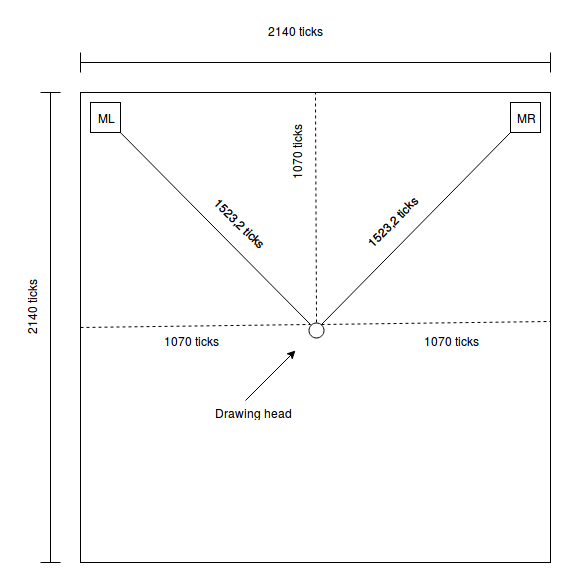
\includegraphics[scale=0.30]{Images/DrawingMachine/Illustration.png}
\caption{ Drawing machine concept. }
\label{OverviewFigure}
\end{figure}

\subsection{Design}
The designing phase of the Drawing Machine has been an iterative process going back and forth until a design was suitable enough for our requirements. Through the trial and error process we learned a lot about how to do better but in many cases also simpler. In some cases we ended up over-engineering solutions only to figure out it would make the whole machine much more complex and could be done much more simple.\\
Figure \ref{OverviewFigure} shows an overview of how we imagine our drawing machine to work. On the figure, the two motor boxes are denoted {\it ML} and {\it MR} for the left and right motor respectively. A box has a piano wire forming a loop to guide the line from a spindle on a shaft of a stepper motor placed in the box. The loop will guide the line from the middle of the spindle down to a part that has a hole towards and close to the whiteboard.
This will keep the line close to the whiteboard and it will be at this point that the line will create an angle towards the drawing pen. It is from this point in both motors and the drawing pen that we say that there is a triangle between the motors and the drawing head. The line will be pulled/released to move the drawing head. The drawing head is pulled down by gravity with the help of a weight.\\ The resulting design of the Drawing Machine is seen in appendix \cref{fig:Images/Jacobselskovsbilleder/IMG 2031.jpg,fig:Images/Jacobselskovsbilleder/IMG 2030.jpg,fig:Images/Jacobselskovsbilleder/IMG 2033.jpg}
The Drawing Machine's stepper motor is set inside two boxes that have nine magnets underneath. The boxes were designed in {\texttt Fusion360} and then laser cut in a 6mm wooden plate (MDF) \footnote{See appendix}. The box is assembled from individual sides of a box by finger joints.   On the stepper motor we designed first a spindle in {\texttt Fusion360} with the idea of solving an issue of the line rolling onto itself. The result of the design is seen in appendix.... but the issue with this solution was the rotation of the spindle. It would draw on the line and then release (rotating in the same direction) giving us a hard time to control it. Instead we did a classic spindle design though with the issue of an error in diameter due to the line rolling onto itself.\\
Next design part was the drawing head. It was important that it was able to not only hold the pen but also tighten (stability). we introduced a wooden block (weight) that kept our pen steady during drawing by pulling the drawing head down. In the beginning we discussed the possibility of the pen being lifted from the board during transport and then pushed to the board when drawing. Because of scope and our artistic interest we chose to let the transport lines be drawn and therefore let the pen stay in the same position all the time.  
\subsection{Mechanics}
The motors of the machine was originally intended to be placed with arbitrary length from one another, but lack of insight resulted in us not being able to assert the exact distance between the motors for an arbitrary setup. There had been ideas to include a load-cell or accelerometers to detect a tightened line between the two motors. This could effectively have been used to assert the distance as a process of homing which results in the motors knowing how long the line is from the given motor to the painting head.\\
This meant that for simplicity we assumed a fixed distance between the motors. {\it Homing} is then used to assert the length of the line from the painting head, to a motor ({\it ML} or {\it MR}, see figure \ref{OverviewFigure}). This is done by placing a reed switch besides each motor such that the line length will be the same when homing to either {\it ML} or {\it MR}, also it should home till the line is as close to zero as possible. Both of these will affect accuracy.\\
The distance between {\it ML} and {\it MR} was measured to be 1070mm and as there are many triangles with two equally lengthen sides, we had to assume a length for the starting position after homing. We set this to 1070mm/2 = 535mm which placed the painting head pretty centered on our whiteboard. 

\subsection{Electronics}
The stepper motors used is model JK42HS34-1334 \footnote{For the lack of a datasheet, see \url{https://www.aliexpress.com/item/10-PCS-NEMA17-stepper-motor-3D-printer-stepper-motor-JK42HS34-1334A-30oz-in-34mm-1-3A/1571641221.html}}. Pay in mind that the numbers found on this site is 1.8 degree per step for the stepper motor. It turns out that our software has been tuned towards a misreading that is 1.3 degree per step. Furthermore, a possible miss communication have made us believe the spindle on the motor to be 2cm in radius, it is in fact 2.5cm. This will be discussed further in the discussion section where the significance of this will be mentioned. The spindle on the motor was believed to be 2cm in radius and the motor turns 1.3 degree each step, we have that $ (2*\pi*2)/360*1.3 = 0.05cm $, which means that the software will know the distance between {\it ML} and {\it MR} not as 1070mm etc., but as $ 1070mm/(0.5mm/step) = 2140 steps $.\\
To control the stepper motors, we will be using two 
"Pololu - A4988 Stepper Motor" Drivers \citep{Pololu:StepperDriver}. These drivers can deliver 1A without a heat-sink. They are therefore needed as one of our stepper motors operate at 1.33A. We were especially made aware of this as the driver hit the 165 degree "Thermal Shutdown Temperature" feature of the driver that is mentioned in the datasheet. This caused noticeable loss of steps. Furthermore since we have two stepper motors, it amounts to over 2A which is the highest current-rated power-source we could acquire. This is however not a consistent load (its maximum), but this can be tolerated by setting the current limiter onboard the Polulu driver such that each stepper only draw 1A each.\\ 
To enable the drawing machine to home. The drawing head will have a magnet attached to the line (same distance on each line from the magnet to the drawing head). To enable the machine to know that this magnet reaches one of the motors {\it ML} or {\it MR} (see \ref{OverviewFigure}), there will be a reed switch placed at the end of the line near {\it ML} and {\it MR}. The electronics aspect of this is the reed switch as well as how to connect it. It is connected to a GPIO logic pin of the Raspberry PI. Any input must have a pull-down resistor to ground aside from the sensor that switches positive power to the pin when triggered. This means that the input pin will either get a direction to ground or a direct connection to positive.\\
The complete schematic of connecting the Polulu boards, steppers, reed switches and Raspberry PI is shown in figure \ref{DrawingMachineSchematic}. Notice also how there is an electrolytic capacitor placed on the motor power source. This is to protect the board against LC voltage spikes \footnote{Polulu board product page. \url{https://www.pololu.com/product/1182}}. We found the driver broke sometimes and we therefore added it which fixed that reliability issue.  \\

\begin{figure}[h]
\centering
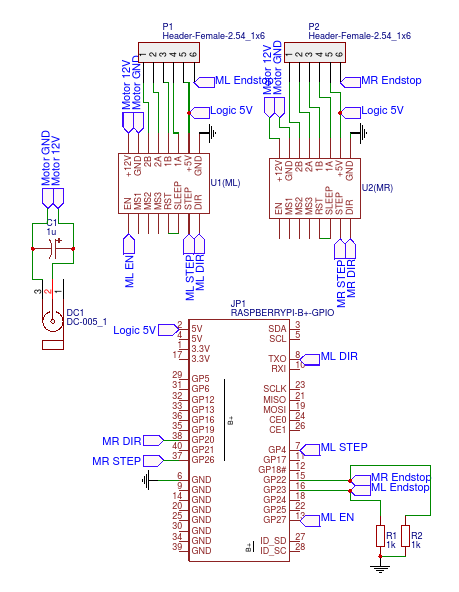
\includegraphics[scale=0.60]{Images/DrawingMachine/Schematic.png}
\caption{ Drawing machine electronics schematic. }
\label{DrawingMachineSchematic}
\end{figure}
 
If we know we want to draw a line from say (0,0) to (10,10), we have to consider that simply telling the motors to adjust their position for the correct line length isn't enough. There are many movements that could travel from A to B and thus to give the illusion of a straight line, we split a line between A and B into a number of coordinates along the line. The amount should just be relative to the resolution of the drawing machine which is 0.78mm per step. This is a problem to be fixed in the software/firmware section.

\subsection{Software/Firmware}
The software is written in python and is aimed at giving one Raspberry PI the capability to segment images into traceable ordered list of coordinates, act as controller for the motors, and to read input from the sensors. This section will describe the most essential aspects of each part.
\\\\
\subsubsection{Segmentation}
The segmentation logic is implemented in one encapsulating python class that takes as instantiating input a path to an image. All images are converted to their gray scale intensities using the {\it Python Image Library}(PIL)\footnote{\url{http://www.pythonware.com/products/pil/}}. Finding pixels to be colored is done using a threshold that defaults to $10$, thereby pixels, $p_{ij}$, are colored if the intensity of $p_{ij}$, $intensity_{ij}$, is such that:
\newline
$intensity_{ij} < threshold\ |\ {0 \leq i < 10, i \in \mathbb{N}}, $
\newline
where the possible intensities is in the range: $[0, 255]$.
For every pixel, $p_{ij}$ that matches this threshold, the segmentation will consider a neighborhood of the surrounding pixels. The size of the neighborhood greatly impacts the final result, since the drawing machine is not capable of lifting the drawing head from the board, and thus draws in one continuous line. This is seen from our simulated experiments with different neighborhoods shown in figure \ref{fig:simulating_experiments}. The simulation is made by plotting each point in an image using {\texttt PIL} rather than sending them as output to any motors. Thereby allowing us to make faster iterative adjustments.
The neighborhood dictates how many adjacent pixels are drawn before the scanning continues which manifests as a {\it transport line} on the final drawing between the last pixel to be colored in the current neighborhood and to the first pixel in the next. Too small of a neighborhood results in more transport lines since less pixels will be considered within the proximity to be drawn and so the scanning will continue to find another pixel to be colored, see figure \ref{subfig:3x3}. On the other hand, a too large neighborhood will result in too many pixels to be considered within the proximity of the currently scanned pixel, thereby the output may seem borderline abstract since otherwise distinct lines are considered the same, an example of this occurs in figure \ref{subfig:100x100}.
\begin{figure}[t]
\caption{Simulated experiments of different segmentation neighborhood sizes}
\label{fig:simulating_experiments}
    \begin{subfigure}[t]{.15\textwidth}
        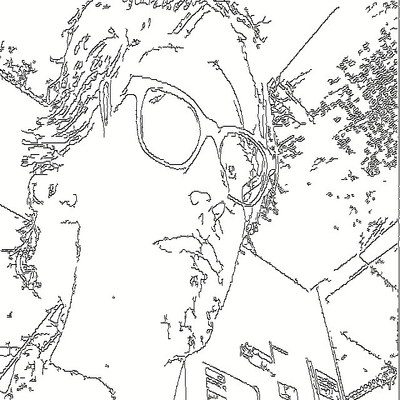
\includegraphics[width=\textwidth]{Images/original_input_resized_400x400.jpg}
        \caption{Original input resized to a fixed $400\times400$}
        \label{subfig:original}
    \end{subfigure}
    \begin{subfigure}[t]{.15\textwidth}
        
\includegraphics[width=\textwidth]{Images/segmented_v1_3x3_neighborhood.png}
        \caption{$3\times3$ neighborhood}
        \label{subfig:3x3}
    \end{subfigure}
    \begin{subfigure}[t]{.15\textwidth}
        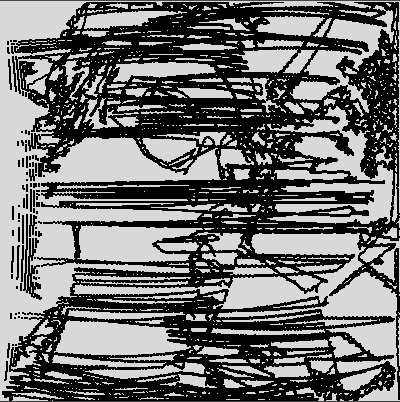
\includegraphics[width=\textwidth]{Images/segmented_v2_5x5_neighborhood.png}
        \caption{$5\times5$ neighborhood}
        \label{subfig:5x5}
    \end{subfigure}
    %next row:
    \begin{subfigure}[t]{.15\textwidth}
        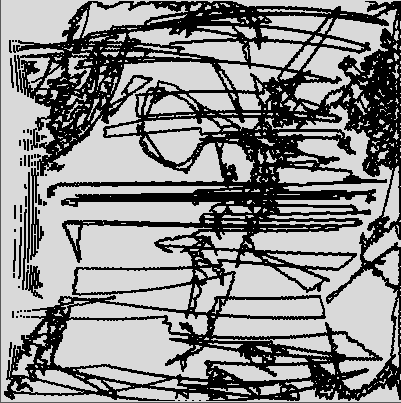
\includegraphics[width=\textwidth]{Images/segmented_v3_7x7_neighborhood.png}
        \caption{$7\times7$ neighborhood}
        \label{subfig:7x7}
    \end{subfigure}
    \begin{subfigure}[t]{.15\textwidth}
        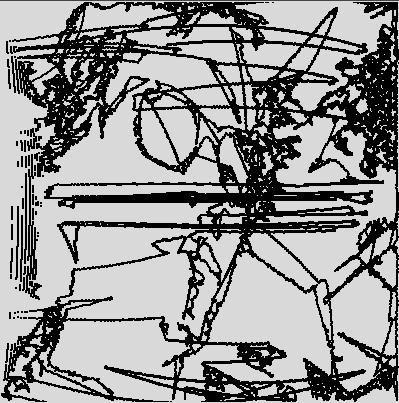
\includegraphics[width=\textwidth]{Images/segmented_v4_9x9_neighborhood.png}
        \caption{$9x9$}
        \label{subfig:9x9}
    \end{subfigure}
    \begin{subfigure}[t]{.15\textwidth}
        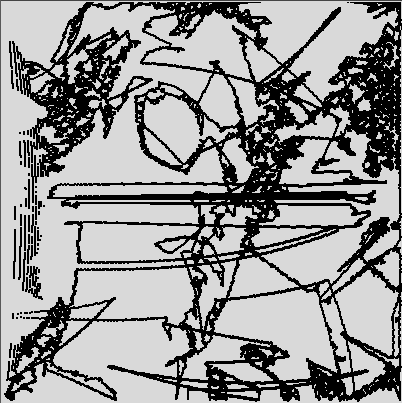
\includegraphics[width=\textwidth]{Images/segmented_v5_11x11_neighborhood.png}
        \caption{$11\times11$ neighborhood}
        \label{subfig:11x11}
    \end{subfigure}
    % last row:
    \begin{subfigure}[t]{.15\textwidth}
        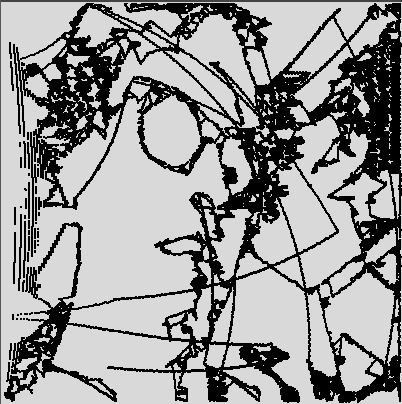
\includegraphics[width=\textwidth]{Images/segmented_v6_22x22_neighborhood.png}
        \caption{$22\times22$ neighborhood}
        \label{subfig:22x22}
    \end{subfigure}
    \begin{subfigure}[t]{.15\textwidth}
        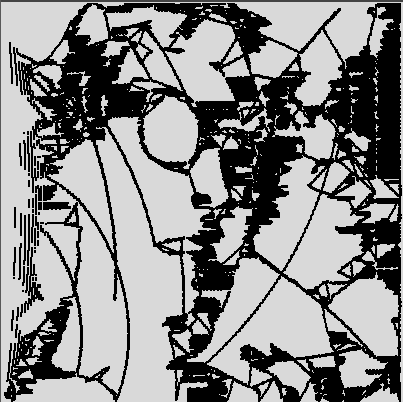
\includegraphics[width=\textwidth]{Images/segmented_v7_47x47_neighborhood.png}
        \caption{$47\times47$ neighborhood}
        \label{subfig:47x47}
    \end{subfigure}
    \begin{subfigure}[t]{.15\textwidth}
        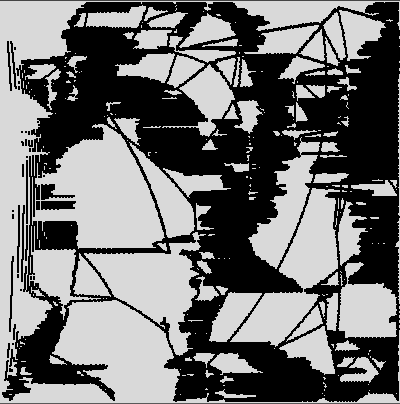
\includegraphics[width=\textwidth]{Images/segmented_v8_100x100_neighborhood.png}
        \caption{$100\times100$ neighborhood}
        \label{subfig:100x100}
    \end{subfigure}
    
\end{figure}

By default we set the size of the neighborhood to be considered a $11\times11$ matrix around the currently considered pixel. The reason for this default size was a trade-off between computation time and an optimal neighborhood size as judged by our simulations. As such, the neighborhood for pixel $p_{ij}$ are the pixels in $\big\{p_{i-2, j-2}, \dotsc, p_{i+2,j+2}\big\}$.
\\\\
\subsubsection{Auto calibration}
For autocalibration, two reed switches, one for each corner, was connected to the Raspberry Pi. The {\it homing} functionality would then first pull the motor up to one corner until the signal from the switch was sent to the Pi, then it would pull the motor to the second corner until a signal was received from the other switch. \\
At each signal, the line length of the corresponding motor was set to $0$. Thereafter, each motor, represented by an instance of a {\texttt Motor} class, is itself responsible for maintaining a counter of the current line length. For simplicity, the line length as well as the dimensions of the coordinate system itself, is measured in stepper motor {\it ticks}. That way, the logic for each motor class would only need to decrement or increment their counter based the direction parameter upon an invocation of their {\texttt tick} method.
\\\\
The implementation for the calibration functionality is largely simplified as two consecutive while loops that is set to continue for as long as no signal is received. Though, one obstacle was that we found that noise could influence a false positive signal being sent prematurely, and so we tackled this logically, by defining the constrain for the {\it while} loops to read $4$ consecutive signals. This approach proved sufficient to filter out false positives signals from the reed switches. 

\subsubsection{Motor control}
The motor control is based on inputs being given as $(x,\ y)$ coordinates and then translating these coordinates into corresponding line length. At the same time, two instantiations of a motor class, as mentioned in the previous section, represents the state of each motor and maintains a counter of the current line length of each line. Given an input $(x,\ y)$ of a desired coordinate to move to, length of the lines $left$ and $right$ is computed as two triangles respectively. That is,
\begin{align}
left  &= \sqrt{x^2 + y^2} \\
right &= \sqrt{(width-x)^2 + y^2} 
\end{align},
for line length {\it left} and {\it right}.
\\\\
After the desired line length is computed, the absolute difference between the current line length of {\it left} and {\it right} and their desired length, is used to know the relative speed needed in order for both adjustments to occur simultaneously.\\
The first iteration of our code, attempted to accommodate for this simultaneous movement through pythons {\it subprocess} library, and then having the motors to be responsible of the delay between each {tick} so that the arrival would match. However, this did not work very wel due to the asynchronous nature of this approach. The {\texttt time.sleep}, which ultimately leaves the scheduling of the frequency of ticks to the operating system to adhere to, was much too imprecise.
\\\\
In the end, everything is run as the same process, and both motors are controlled via the same {\it while} loop. A timestamp is assigned to each motor which is updated everytime a motor is asked to {\it tick}. Then comparing the timestamp for each motor with the current, the motor is asked to move when the frequency, measured in time, is smaller than the time delta. To avoid rounding errors, a method, {\it approx}, is used to measure whether the current line length is within one tick of the desired length. This prevents to motor going on endlessly moving back and forth.

% \begin{figure}
% \begin{python}
% def getNextLineLength(self, next_pos):                                                                             
%     """ Given the next coordinate set, next_pos,                                                   
%         compute the lenght of the line for motorRight                                         
%         and motorLeft                                    
%     """                                                                
%     x, y = next_pos                                                                              
%     # compute left triangle:                                                                  
%     left  = math.sqrt(x**2 + y**2)                                                         
%     # compute right triangle:                                                   
%     right = math.sqrt((self.width - x)**2 + y**2)

%     return left, right
% \end{python}
% \caption{Code snippet showing the computation of next line length given a coordinate set, {\it next\_pos}}
% \label{fig:compute_line_length_code}
% \end{figure}

%Group Report Information: Did it work properly? What kind of tests did you run to test your prototype? Could you provide some data that shows the performance of the prototype (speed, success rate, etc.)?

\section{Results/Analysis}

%Group Report Information: What are the strengths and shortcomings of your device? Did it match the requirements?  How would you improve/develop it further, if you had time?

\section{Discussion} 
\subsection{Improvement}
\subsubsection{Homing offset}
To improve on the inaccurate measurement of the wire length, there could be a number of different ways to improve it. One would be to add stronger stepper motors and the reason for that is that we are limited in how close the drawing head can be to head without assistance from the other motor. This means that the end-stop magnet is placed with a length from the drawing head (on the wire) that is relative to what was possible by trial and error. A stronger stepper motor could pull the drawing head as close to the motor as possible to allow for more accurate measurement of wire length and stronger stepper motors would also improve the possibilities of speed. \\
Another and perhaps better way is to measure the line width from the magnet to the drawing head and hard-code it in the software/firmware. This would improve accuracy, but not speed limitation unlike the change of stepper motor.

\subsubsection{Reed switch placement}
We have taped the reed switch to the whiteboard which is a quite unprofessional and cheap way. It makes it fragile and it hurts accuracy when they displaces and thus does not trigger only when the endstop magnet gets to the very end. Thus it would be a wise improvement to add a 3D printed holder that would hold it in place against the motorbox.

\subsubsection{Motorbox distance}
The distance between the motors are fixed at the moment in software. To allow for estimation of the wire length between the motors, we could do so if we knew when the wires are tight. This could be observed using an accelerate or a load cell. A load cell could detect it if the wire went though a hole in the load-cell, then if the wire is tight, it won't hang and thus won't push downwards as much. The accelerometer could be placed on the wire to measure angle.

\subsubsection{Including ideas from other similar projects}
Our finding of more background material late in the process showed that instead of using spindles, we could have used a pulley-like setup \citep{Vimio:2010:DrawingMachine}. Doing so could have improved accuracy by the spindle not increasing in diameter as a result of wire lying on top of each other. This can seriously affect accuracy as it changes the rate of wire pulled/release per step. With shorter wire we have reduced the significance of this problem, but it must definitely be causing skewed movement. 
  
 

% An example of a floating figure using the graphicx package.
% Note that \label must occur AFTER (or within) \caption.
% For figures, \caption should occur after the \includegraphics.
% Note that IEEEtran v1.7 and later has special internal code that
% is designed to preserve the operation of \label within \caption
% even when the captionsoff option is in effect. However, because
% of issues like this, it may be the safest practice to put all your
% \label just after \caption rather than within \caption{}.
%
% Reminder: the "draftcls" or "draftclsnofoot", not "draft", class
% option should be used if it is desired that the figures are to be
% displayed while in draft mode.
%
%\begin{figure}[!t]
%\centering
%\includegraphics[width=2.5in]{myfigure}
% where an .eps filename suffix will be assumed under latex, 
% and a .pdf suffix will be assumed for pdflatex; or what has been declared
% via \DeclareGraphicsExtensions.
%\caption{Simulation results for the network.}
%\label{fig_sim}
%\end{figure}

% Note that IEEE typically puts floats only at the top, even when this
% results in a large percentage of a column being occupied by floats.


% An example of a double column floating figure using two subfigures.
% (The subfig.sty package must be loaded for this to work.)
% The subfigure \label commands are set within each subfloat command,
% and the \label for the overall figure must come after \caption.
% \hfil is used as a separator to get equal spacing.
% Watch out that the combined width of all the subfigures on a 
% line do not exceed the text width or a line break will occur.
%
%\begin{figure*}[!t]
%\centering
%\subfloat[Case I]{\includegraphics[width=2.5in]{box}%
%\label{fig_first_case}}
%\hfil
%\subfloat[Case II]{\includegraphics[width=2.5in]{box}%
%\label{fig_second_case}}
%\caption{Simulation results for the network.}
%\label{fig_sim}
%\end{figure*}
%
% Note that often IEEE papers with subfigures do not employ subfigure
% captions (using the optional argument to \subfloat[]), but instead will
% reference/describe all of them (a), (b), etc., within the main caption.
% Be aware that for subfig.sty to generate the (a), (b), etc., subfigure
% labels, the optional argument to \subfloat must be present. If a
% subcaption is not desired, just leave its contents blank,
% e.g., \subfloat[].


% An example of a floating table. Note that, for IEEE style tables, the
% \caption command should come BEFORE the table and, given that table
% captions serve much like titles, are usually capitalized except for words
% such as a, an, and, as, at, but, by, for, in, nor, of, on, or, the, to
% and up, which are usually not capitalized unless they are the first or
% last word of the caption. Table text will default to \footnotesize as
% IEEE normally uses this smaller font for tables.
% The \label must come after \caption as always.
%
%\begin{table}[!t]
%% increase table row spacing, adjust to taste
%\renewcommand{\arraystretch}{1.3}
% if using array.sty, it might be a good idea to tweak the value of
% \extrarowheight as needed to properly center the text within the cells
%\caption{An Example of a Table}
%\label{table_example}
%\centering
%% Some packages, such as MDW tools, offer better commands for making tables
%% than the plain LaTeX2e tabular which is used here.
%\begin{tabular}{|c||c|}
%\hline
%One & Two\\
%\hline
%Three & Four\\
%\hline
%\end{tabular}
%\end{table}


% Note that the IEEE does not put floats in the very first column
% - or typically anywhere on the first page for that matter. Also,
% in-text middle ("here") positioning is typically not used, but it
% is allowed and encouraged for Computer Society conferences (but
% not Computer Society journals). Most IEEE journals/conferences use
% top floats exclusively. 
% Note that, LaTeX2e, unlike IEEE journals/conferences, places
% footnotes above bottom floats. This can be corrected via the
% \fnbelowfloat command of the stfloats package.



%Group Report Information: No notes

\section{Conclusion}
%Creating a drawing machine is not a novel idea, so the result itself was never a goal in and on itself. That said, the fact that we have been able to create a machinery that creates recognizable drawings on a physical whiteboard is very rewarding. Thereby, the resulting product is much more capable than we could have hoped for. Even if many sources of errors still remains.
In conclusion creating a drawing machine is not something new or a novel idea. It has been done by many and in many different ways. We chose to do it our own way and try and fail as much as we could in order to learn. Inspiration from others work would definitely have drawn the project in other direction and maybe solved some errors or been more efficient. But with the trial and error came learning and in the end our machine.\\
We would like to work further on this project making it more smooth and less of a prototype. We have in the finale phase thought of many new ways to limit errors and control variable. At the same time many new features could be added. We have a JeVois smart camera\footnote{http://jevois.org/} that can detect edges and would be a cool implementation to the project. The Drawing Machine would then draw what the camera was seeing.  




% conference papers do not normally have an appendix


% use section* for acknowledgment 

% trigger a \newpage just before the given reference
% number - used to balance the columns on the last page
% adjust value as needed - may need to be readjusted if
% the document is modified later
%\IEEEtriggeratref{8}
% The "triggered" command can be changed if desired:
%\IEEEtriggercmd{\enlargethispage{-5in}}

% references section
\bibliography{Sections/References}
%% can use a bibliography generated by BibTeX as a .bbl file
% BibTeX documentation can be easily obtained at:
% http://www.ctan.org/tex-archive/biblio/bibtex/contrib/doc/
% The IEEEtran BibTeX style support page is at:
% http://www.michaelshell.org/tex/ieeetran/bibtex/
%\bibliographystyle{IEEEtran}
% argument is your BibTeX string definitions and bibliography database(s)
%\bibliography{IEEEabrv,../bib/paper}
%
% <OR> manually copy in the resultant .bbl file
% set second argument of \begin to the number of references
% (used to reserve space for the reference number labels box)

%Group Report Information: You can add references, but they are not needed. (All the parts used in your project should be documented in the annexes.)
\begin{thebibliography}{1}

\bibitem{IEEEhowto:kopka}
H.~Kopka and P.~W. Daly, \emph{A Guide to \LaTeX}, 3rd~ed.\hskip 1em plus
  0.5em minus 0.4em\relax Harlow, England: Addison-Wesley, 1999.

\end{thebibliography}
 

%Group Report Information: Bill of materials (BOM): What do you need to build your prototype? List all the parts that you device contains. If you develop electronics, you should have a BOM for the electronics and another for the mechanics. The BOM of the electronics can be generated from most ECAD programs automatically.

\appendix

\section{Some Appendix}
\label{whatever}
The contents...
%%%%%%%%%%%%%%%%%%%%%%%%%%%%%%%%%%%%%%%%%%%%%%%%%%%%%%%%%%%%%%%%%%%%%%%%%%%%%%%%
\begin{figure}[H]
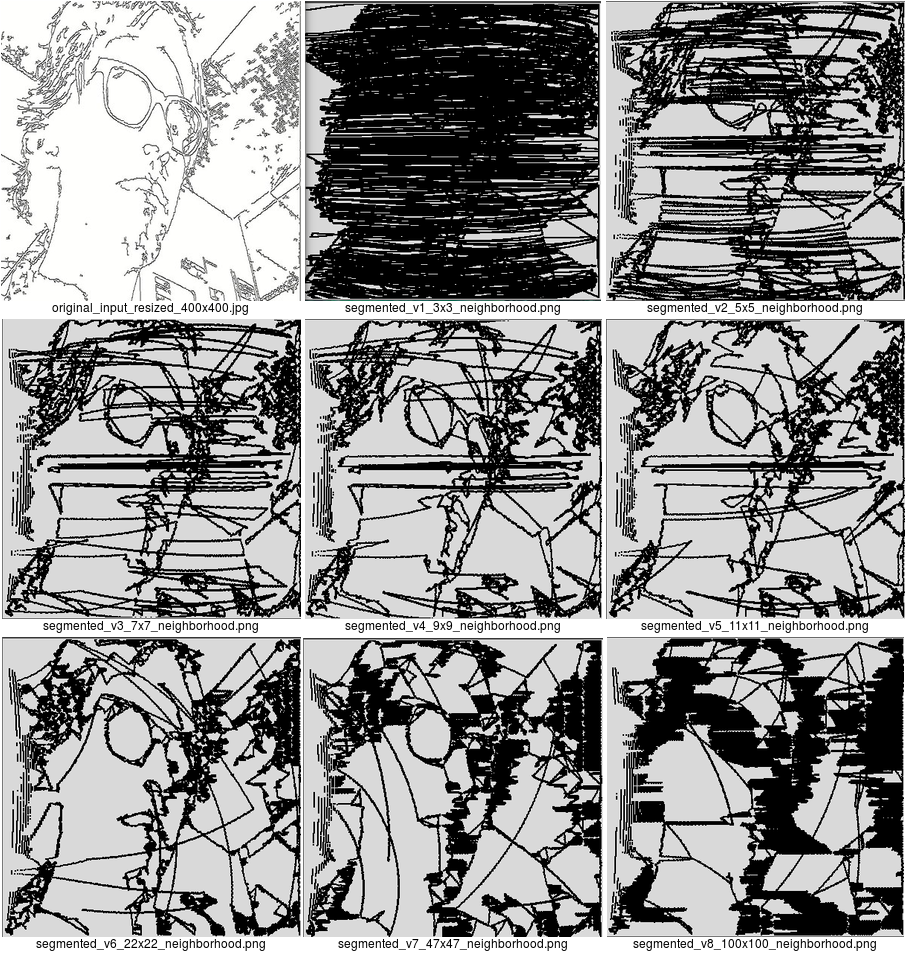
\includegraphics[width=\textwidth]{Images/segmentations_overview.png}
\caption{Images/segmentations overview.png}
\label{fig:Images/segmentations overview.png}
\end{figure}
%%%%%%%%%%%%%%%%%%%%%%%%%%%%%%%%%%%%%%%%%%%%%%%%%%%%%%%%%%%%%%%%%%%%%%%%%%%%%%%%
\begin{figure}[H]
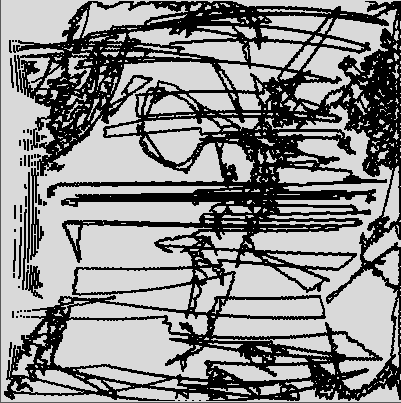
\includegraphics[width=\textwidth]{Images/segmented_v3_7x7_neighborhood.png}
\caption{Images/segmented v3 7x7 neighborhood.png}
\label{fig:Images/segmented v3 7x7 neighborhood.png}
\end{figure}
% %%%%%%%%%%%%%%%%%%%%%%%%%%%%%%%%%%%%%%%%%%%%%%%%%%%%%%%%%%%%%%%%%%%%%%%%%%%%%%%%
% \begin{figure}[H]
% 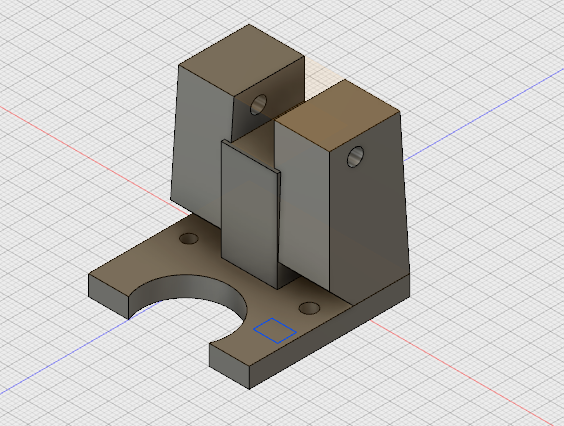
\includegraphics[width=\textwidth]{Images/Screen Shot 2017-12-13 at 14.16.47.png}
% \caption{Images/Screen Shot 2017-12-13 at 14.16.47.png}
% \label{fig:Images/Screen Shot 2017-12-13 at 14.16.47.png}
% \end{figure}
%%%%%%%%%%%%%%%%%%%%%%%%%%%%%%%%%%%%%%%%%%%%%%%%%%%%%%%%%%%%%%%%%%%%%%%%%%%%%%%%
\begin{figure}[H]
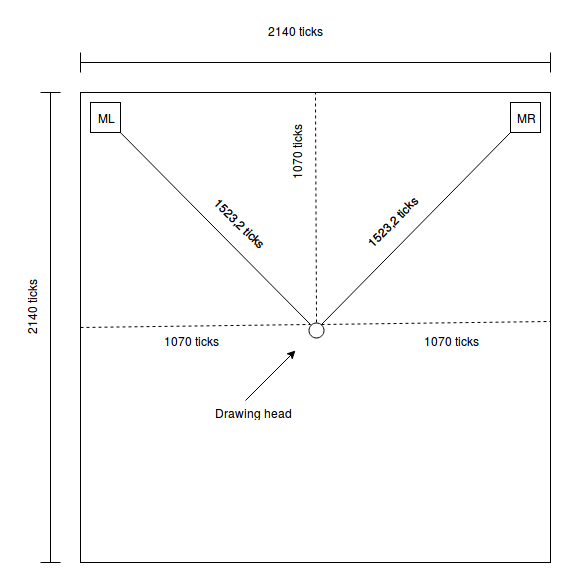
\includegraphics[width=\textwidth]{Images/DrawingMachine/Illustration.png}
\caption{Images/DrawingMachine/Illustration.png}
\label{fig:Images/DrawingMachine/Illustration.png}
\end{figure}
%%%%%%%%%%%%%%%%%%%%%%%%%%%%%%%%%%%%%%%%%%%%%%%%%%%%%%%%%%%%%%%%%%%%%%%%%%%%%%%%
\begin{figure}[H]
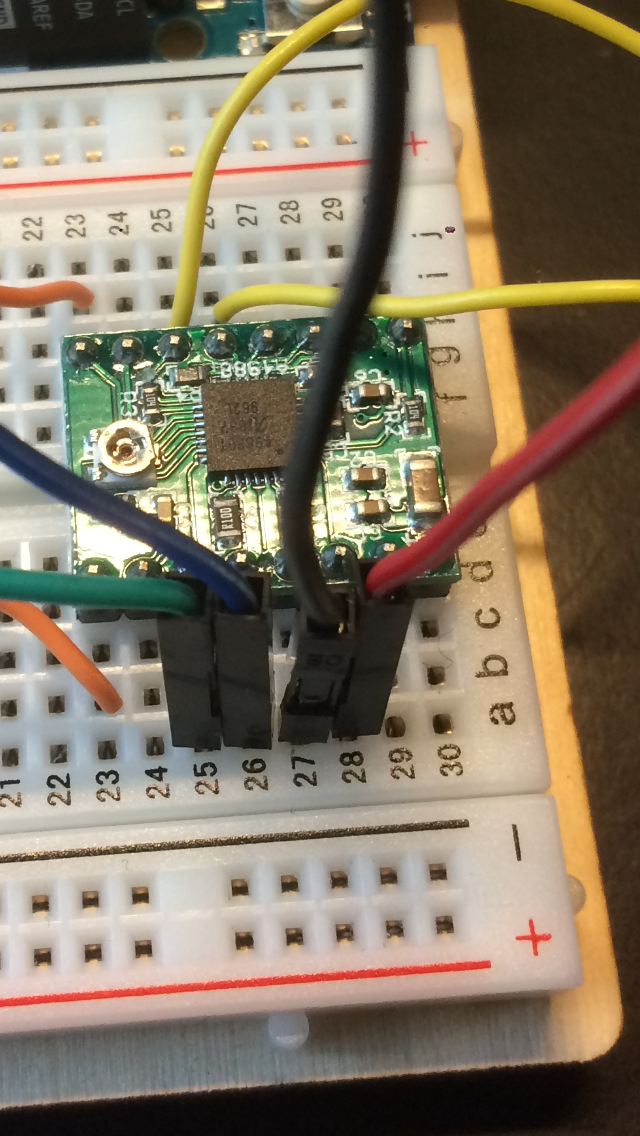
\includegraphics[width=\textwidth]{Images/DrawingMachine/IMG_0898.PNG}
\caption{Images/DrawingMachine/IMG 0898.PNG}
\label{fig:Images/DrawingMachine/IMG 0898.PNG}
\end{figure}
%%%%%%%%%%%%%%%%%%%%%%%%%%%%%%%%%%%%%%%%%%%%%%%%%%%%%%%%%%%%%%%%%%%%%%%%%%%%%%%%
\begin{figure}[H]
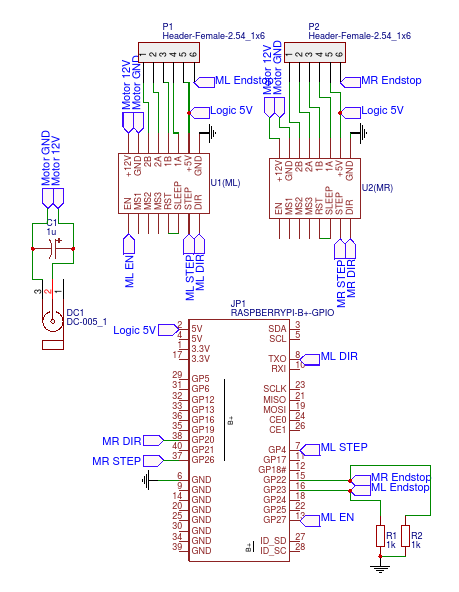
\includegraphics[width=\textwidth]{Images/DrawingMachine/Schematic.png}
\caption{Images/DrawingMachine/Schematic.png}
\label{fig:Images/DrawingMachine/Schematic.png}
\end{figure}
%%%%%%%%%%%%%%%%%%%%%%%%%%%%%%%%%%%%%%%%%%%%%%%%%%%%%%%%%%%%%%%%%%%%%%%%%%%%%%%%
% \begin{figure}[H]
% 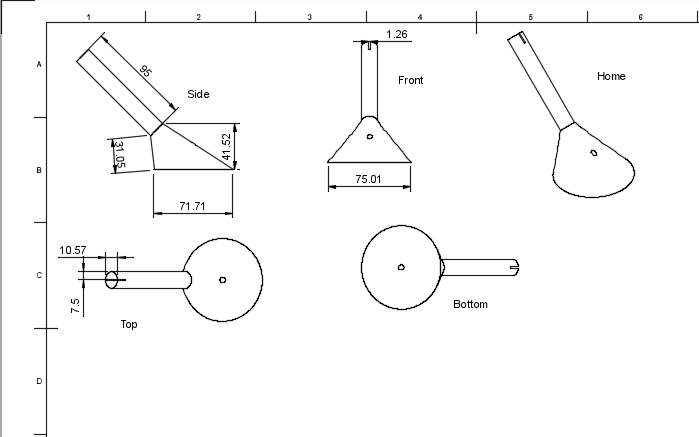
\includegraphics[width=\textwidth]{Images/Screen Shot 2017-12-13 at 13.44.19.png}
% \caption{Images/Screen Shot 2017-12-13 at 13.44.19.png}
% \label{fig:Images/Screen Shot 2017-12-13 at 13.44.19.png}
% \end{figure}
%%%%%%%%%%%%%%%%%%%%%%%%%%%%%%%%%%%%%%%%%%%%%%%%%%%%%%%%%%%%%%%%%%%%%%%%%%%%%%%%
\begin{figure}[H]
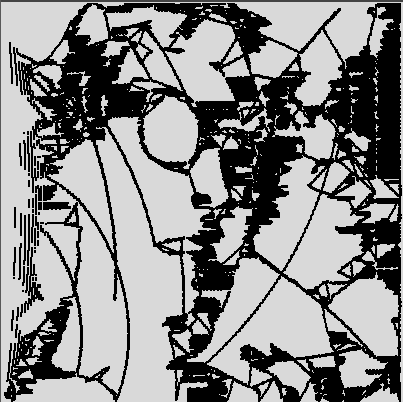
\includegraphics[width=\textwidth]{Images/segmented_v7_47x47_neighborhood.png}
\caption{Images/segmented v7 47x47 neighborhood.png}
\label{fig:Images/segmented v7 47x47 neighborhood.png}
\end{figure}
%%%%%%%%%%%%%%%%%%%%%%%%%%%%%%%%%%%%%%%%%%%%%%%%%%%%%%%%%%%%%%%%%%%%%%%%%%%%%%%%
% \begin{figure}[H]
% 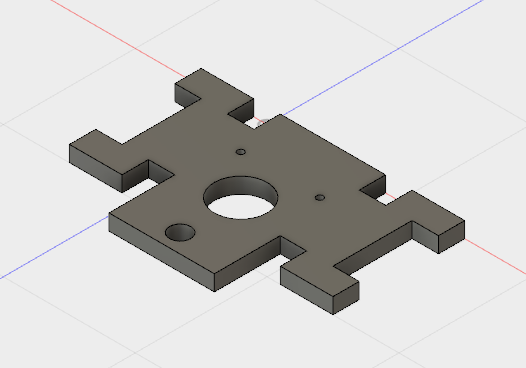
\includegraphics[width=\textwidth]{Images/Screen Shot 2017-12-13 at 14.15.38.png}
% \caption{Images/Screen Shot 2017-12-13 at 14.15.38.png}
% \label{fig:Images/Screen Shot 2017-12-13 at 14.15.38.png}
% \end{figure}
%%%%%%%%%%%%%%%%%%%%%%%%%%%%%%%%%%%%%%%%%%%%%%%%%%%%%%%%%%%%%%%%%%%%%%%%%%%%%%%%
% \begin{figure}[H]
% 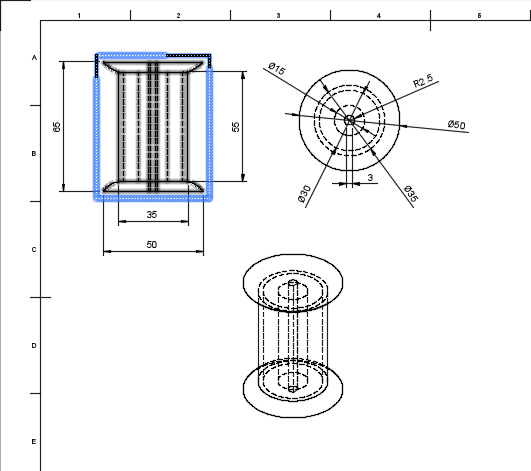
\includegraphics[width=\textwidth]{Images/Screen Shot 2017-12-13 at 12.48.59.png}
% \caption{Images/Screen Shot 2017-12-13 at 12.48.59.png}
% \label{fig:Images/Screen Shot 2017-12-13 at 12.48.59.png}
% \end{figure}
%%%%%%%%%%%%%%%%%%%%%%%%%%%%%%%%%%%%%%%%%%%%%%%%%%%%%%%%%%%%%%%%%%%%%%%%%%%%%%%%
\begin{figure}[H]
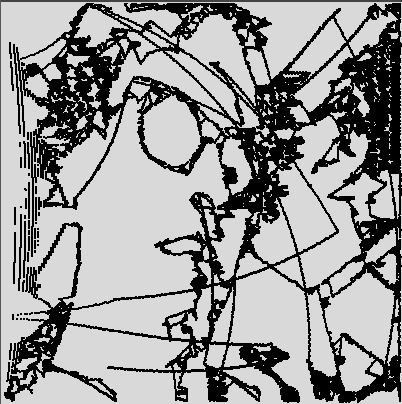
\includegraphics[width=\textwidth]{Images/segmented_v6_22x22_neighborhood.png}
\caption{Images/segmented v6 22x22 neighborhood.png}
\label{fig:Images/segmented v6 22x22 neighborhood.png}
\end{figure}
%%%%%%%%%%%%%%%%%%%%%%%%%%%%%%%%%%%%%%%%%%%%%%%%%%%%%%%%%%%%%%%%%%%%%%%%%%%%%%%%
% \begin{figure}[H]
% 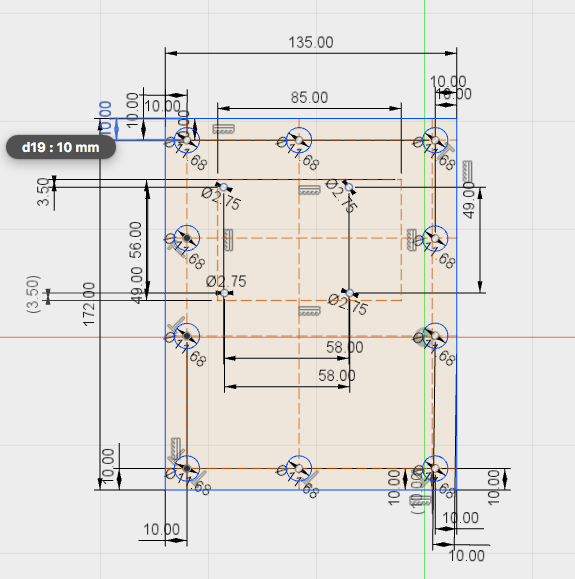
\includegraphics[width=\textwidth]{Images/Screen Shot 2017-12-13 at 12.38.38.png}
% \caption{Images/Screen Shot 2017-12-13 at 12.38.38.png}
% \label{fig:Images/Screen Shot 2017-12-13 at 12.38.38.png}
% \end{figure}
%%%%%%%%%%%%%%%%%%%%%%%%%%%%%%%%%%%%%%%%%%%%%%%%%%%%%%%%%%%%%%%%%%%%%%%%%%%%%%%%
% \begin{figure}[H]
% 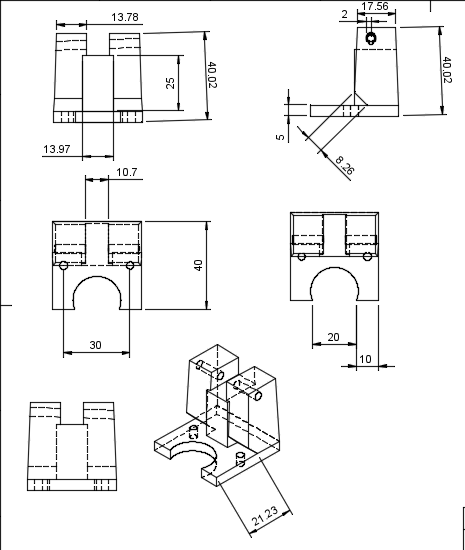
\includegraphics[width=\textwidth]{Images/Screen Shot 2017-12-13 at 14.12.59.png}
% \caption{Images/Screen Shot 2017-12-13 at 14.12.59.png}
% \label{fig:Images/Screen Shot 2017-12-13 at 14.12.59.png}
% \end{figure}
%%%%%%%%%%%%%%%%%%%%%%%%%%%%%%%%%%%%%%%%%%%%%%%%%%%%%%%%%%%%%%%%%%%%%%%%%%%%%%%%
\begin{figure}[H]
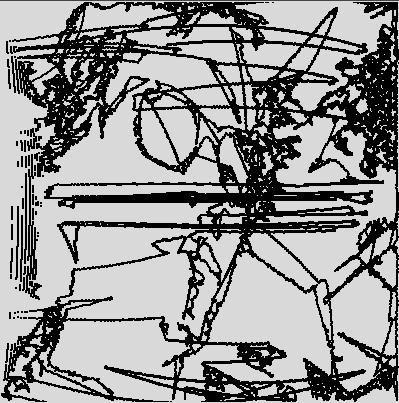
\includegraphics[width=\textwidth]{Images/segmented_v4_9x9_neighborhood.png}
\caption{Images/segmented v4 9x9 neighborhood.png}
\label{fig:Images/segmented v4 9x9 neighborhood.png}
\end{figure}
%%%%%%%%%%%%%%%%%%%%%%%%%%%%%%%%%%%%%%%%%%%%%%%%%%%%%%%%%%%%%%%%%%%%%%%%%%%%%%%%
% \begin{figure}[H]
% 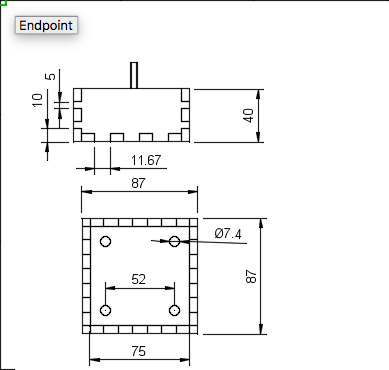
\includegraphics[width=\textwidth]{Images/Screen Shot 2017-12-13 at 15.23.56.png}
% \caption{Images/Screen Shot 2017-12-13 at 15.23.56.png}
% \label{fig:Images/Screen Shot 2017-12-13 at 15.23.56.png}
% \end{figure}
%%%%%%%%%%%%%%%%%%%%%%%%%%%%%%%%%%%%%%%%%%%%%%%%%%%%%%%%%%%%%%%%%%%%%%%%%%%%%%%%
% \begin{figure}[H]
% 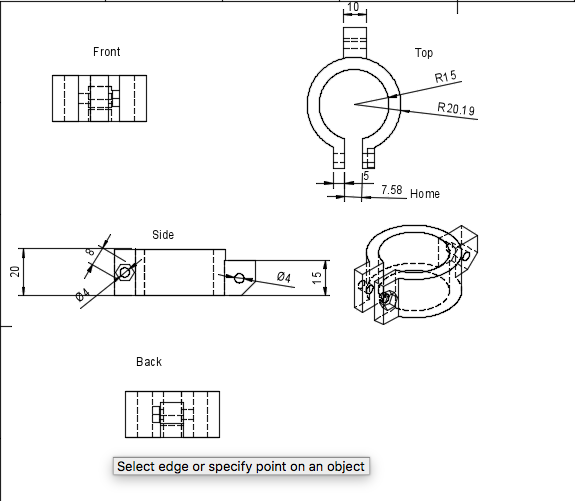
\includegraphics[width=\textwidth]{Images/Screen Shot 2017-12-13 at 13.25.34.png}
% \caption{Images/Screen Shot 2017-12-13 at 13.25.34.png}
% \label{fig:Images/Screen Shot 2017-12-13 at 13.25.34.png}
% \end{figure}
%%%%%%%%%%%%%%%%%%%%%%%%%%%%%%%%%%%%%%%%%%%%%%%%%%%%%%%%%%%%%%%%%%%%%%%%%%%%%%%%
% \begin{figure}[H]
% 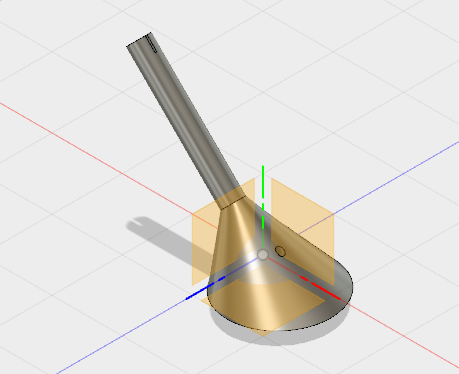
\includegraphics[width=\textwidth]{Images/Screen Shot 2017-12-13 at 14.16.05.png}
% \caption{Images/Screen Shot 2017-12-13 at 14.16.05.png}
% \label{fig:Images/Screen Shot 2017-12-13 at 14.16.05.png}
% \end{figure}
%%%%%%%%%%%%%%%%%%%%%%%%%%%%%%%%%%%%%%%%%%%%%%%%%%%%%%%%%%%%%%%%%%%%%%%%%%%%%%%%
\begin{figure}[H]

\includegraphics[width=\textwidth]{Images/segmented_v1_3x3_neighborhood.png}
\caption{Images/segmented v1 3x3 neighborhood.png}
\label{fig:Images/segmented v1 3x3 neighborhood.png}
\end{figure}
%%%%%%%%%%%%%%%%%%%%%%%%%%%%%%%%%%%%%%%%%%%%%%%%%%%%%%%%%%%%%%%%%%%%%%%%%%%%%%%%
% \begin{figure}[H]
% 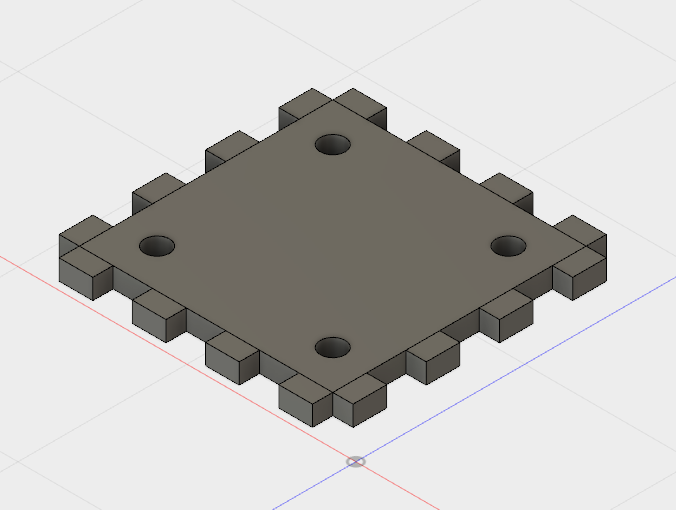
\includegraphics[width=\textwidth]{Images/Screen Shot 2017-12-13 at 14.59.03.png}
% \caption{Images/Screen Shot 2017-12-13 at 14.59.03.png}
% \label{fig:Images/Screen Shot 2017-12-13 at 14.59.03.png}
% \end{figure}
%%%%%%%%%%%%%%%%%%%%%%%%%%%%%%%%%%%%%%%%%%%%%%%%%%%%%%%%%%%%%%%%%%%%%%%%%%%%%%%%
\begin{figure}[H]
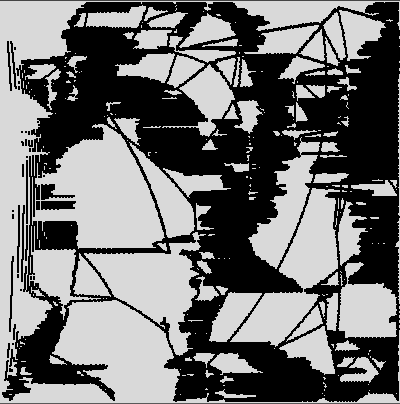
\includegraphics[width=\textwidth]{Images/segmented_v8_100x100_neighborhood.png}
\caption{Images/segmented v8 100x100 neighborhood.png}
\label{fig:Images/segmented v8 100x100 neighborhood.png}
\end{figure}
%%%%%%%%%%%%%%%%%%%%%%%%%%%%%%%%%%%%%%%%%%%%%%%%%%%%%%%%%%%%%%%%%%%%%%%%%%%%%%%%
\begin{figure}[H]
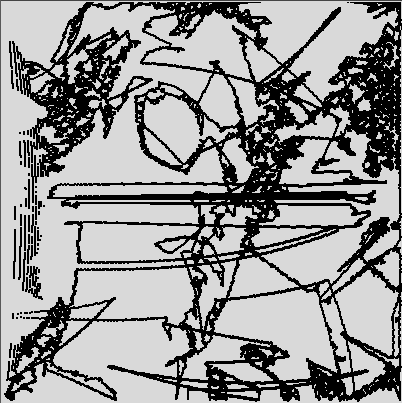
\includegraphics[width=\textwidth]{Images/segmented_v5_11x11_neighborhood.png}
\caption{Images/segmented v5 11x11 neighborhood.png}
\label{fig:Images/segmented v5 11x11 neighborhood.png}
\end{figure}
%%%%%%%%%%%%%%%%%%%%%%%%%%%%%%%%%%%%%%%%%%%%%%%%%%%%%%%%%%%%%%%%%%%%%%%%%%%%%%%%
% \begin{figure}[H]
% 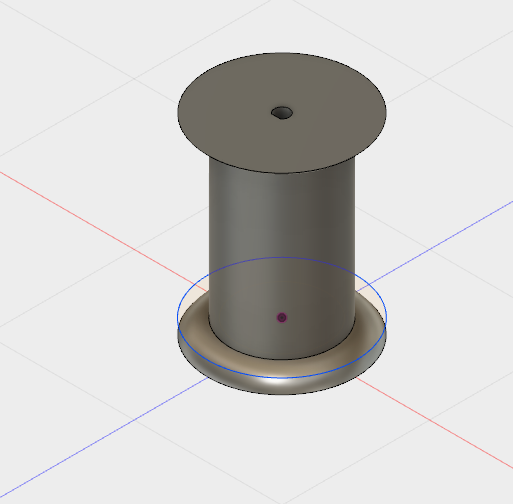
\includegraphics[width=\textwidth]{Images/Screen Shot 2017-12-13 at 12.42.31.png}
% \caption{Images/Screen Shot 2017-12-13 at 12.42.31.png}
% \label{fig:Images/Screen Shot 2017-12-13 at 12.42.31.png}
% \end{figure}
%%%%%%%%%%%%%%%%%%%%%%%%%%%%%%%%%%%%%%%%%%%%%%%%%%%%%%%%%%%%%%%%%%%%%%%%%%%%%%%%
% \begin{figure}[H]
% 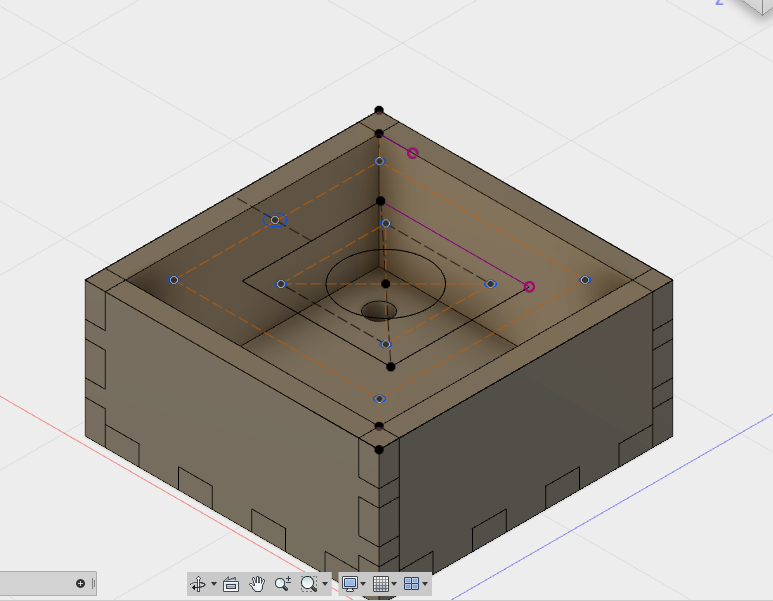
\includegraphics[width=\textwidth]{Images/Screen Shot 2017-12-13 at 15.00.38.png}
% \caption{Images/Screen Shot 2017-12-13 at 15.00.38.png}
% \label{fig:Images/Screen Shot 2017-12-13 at 15.00.38.png}
% \end{figure}
%%%%%%%%%%%%%%%%%%%%%%%%%%%%%%%%%%%%%%%%%%%%%%%%%%%%%%%%%%%%%%%%%%%%%%%%%%%%%%%%
\begin{figure}[H]
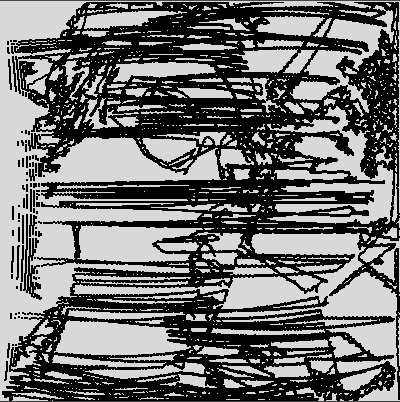
\includegraphics[width=\textwidth]{Images/segmented_v2_5x5_neighborhood.png}
\caption{Images/segmented v2 5x5 neighborhood.png}
\label{fig:Images/segmented v2 5x5 neighborhood.png}
\end{figure}
%%%%%%%%%%%%%%%%%%%%%%%%%%%%%%%%%%%%%%%%%%%%%%%%%%%%%%%%%%%%%%%%%%%%%%%%%%%%%%%%
% \begin{figure}[H]
% 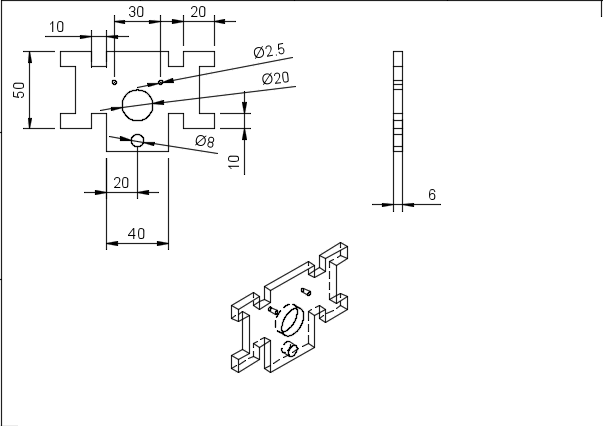
\includegraphics[width=\textwidth]{Images/Screen Shot 2017-12-13 at 13.53.09.png}
% \caption{Images/Screen Shot 2017-12-13 at 13.53.09.png}
% \label{fig:Images/Screen Shot 2017-12-13 at 13.53.09.png}
% \end{figure}
%%%%%%%%%%%%%%%%%%%%%%%%%%%%%%%%%%%%%%%%%%%%%%%%%%%%%%%%%%%%%%%%%%%%%%%%%%%%%%%%
% \begin{figure}[H]
% 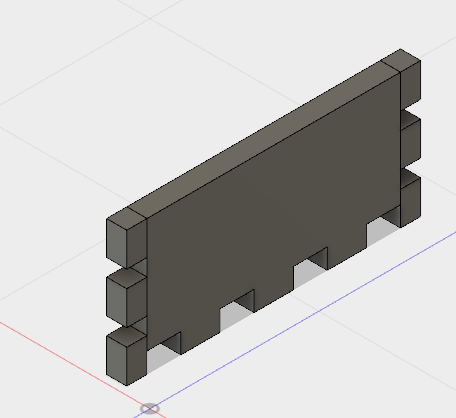
\includegraphics[width=\textwidth]{Images/Screen Shot 2017-12-13 at 14.59.11.png}
% \caption{Images/Screen Shot 2017-12-13 at 14.59.11.png}
% \label{fig:Images/Screen Shot 2017-12-13 at 14.59.11.png}
% \end{figure}
%%%%%%%%%%%%%%%%%%%%%%%%%%%%%%%%%%%%%%%%%%%%%%%%%%%%%%%%%%%%%%%%%%%%%%%%%%%%%%%%
% \begin{figure}[H]
% 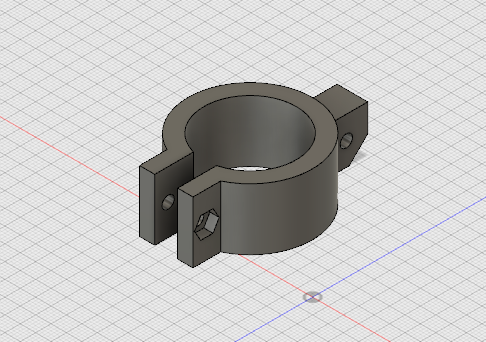
\includegraphics[width=\textwidth]{Images/Screen Shot 2017-12-13 at 14.16.21.png}
% \caption{Images/Screen Shot 2017-12-13 at 14.16.21.png}
% \label{fig:Images/Screen Shot 2017-12-13 at 14.16.21.png}
% \end{figure}
 

% that's all folks
\end{document}


